%~~~~~~~~~~~~~~~~~~~~~~~~~~~~~~~~~~~~~~~~~~~~~~~~~~~~~~~~~~~~~~~~~~~~~~~
\chapter{Representação probabilística de grafos}\label{cap:graphs}
%~~~~~~~~~~~~~~~~~~~~~~~~~~~~~~~~~~~~~~~~~~~~~~~~~~~~~~~~~~~~~~~~~~~~~~~

Estruturas de dados probabilísticas apresentam novas formas de resolver problemas clássicos sob um ponto de vista probabilístico. Apresentaremos, neste capítulo, ideias para representações probabilísticas de grafos utilizando estruturas descritas nos capítulos anteriores.

Spinrad mostra em \cite{spinrad2003efficient} que $\Theta(n^2)$ bits são necessários para representar qualquer grafo através da clássica representação de grafos por matriz de adjacência. Classes específicas de grafos, entretanto, podem possuir representações mais compactas. Introduzimos a teoria sobre representações eficientes, bem como a definição de representações implícitas, ótimas ao longo da Seção~\ref{sec:graphs:implicit}.

Estruturas probabilísticas possuem grande aplicabilidade em bioinformática. Os resultados em \cite{pell2012scaling}, \cite{zhang2014these}, \cite{ondov2016mash} e \cite{junior2016efficient} mostram o uso das estruturas probabilísticas discutidas ao longo deste trabalho em diversos passos na montagem de fragmentos de genoma bacterial. Apresentamos em detalhe a construção de uma representação probabilística baseada em filtros de Bloom para grafos \emph{de Bruijn} na Seção~\ref{sec:graphs:example}.

Por fim, apresentamos novas ideias para representação implícita probabilística de grafos gerais, bem como de alguma subclasses específicas nas Seções~\ref{sec:graphs:bloom} e \ref{sec:graphs:countmin}.

\section{Introdução a representações eficientes}\label{sec:graphs:implicit}

Nesta seção, apresentamos conceitos sobre representações eficientes de grafos. Esta área baseia-se muito nos trabalhos de Muller \cite{muller1988local} e Kannan, Naor e Rudich \cite{kannan1992implicat}, entretanto, o livro de Spinrad \cite{spinrad2003efficient} sintetizou bem a teoria descrita até o momento, motivando novos trabalhos na área.

Para fins de notação, dizemos que um grafo $G$ é denotado pela tupla $(V, E)$, onde $V$ é o conjunto de vértices, de cardinalidade $n = |V|$ e $E$ é o conjunto de arestas, de cardinalidade $m = |E|$. Cada aresta é um par não-ordenado $(u, v) com u,v \in V$. A maior parte das discussões nesta seção aplicam-se a grafos rotulados (onde grafos isomorfos com rótulos diferentes são considerados grafos diferentes).

Começamos por discutir as duas representações clássicas de grafos: matriz de adjacência e lista de adjacência. Na discussão que se segue, está implícito o fato de que para para nomear com cadeias binárias os elementos de um conjunto contendo N elementos, é necessário e suficiente utilizar cadeias de tamanho $O(\log N)$.

A matriz de adjacência utiliza $\Theta(n^2)$ bits para representar a presença ou ausência cada uma das possíveis arestas entre dois vértices no grafo. A estrutura possui este nome pois consiste de uma matriz binária $M$ de dimensão $n \times n$ onde $M[u,v] = 1$ se e somente se os vértices $u,v$ são adjacentes (assume-se $V = [1..n]$). A vantagem desta representação é a possibilidade de testar a adjacência entre dois vértices em tempo constante.

A lista de adjacência mantém, para cada vértice $v$, uma lista encadeada dos vértices $u$ tal que $(u, v) \in E$. Para representar um grafo, $n$ listas são mantidas com um total de $2m$ itens (pois cada aresta é representada em exatamente duas listas). Cada item pode ser denotado por um natural no intervalo $[1;n]$ para representar o vértice e outro natural no intervalo $[1;2m]$ para servir de apontador para o próximo item, precisando, portanto de $O(\log n + \log m) = O(\log n)$ bits para ser representado. Assim, a lista de adjacência representa um grafo de $n$ vértices utilizando $O(m \log n)$ bits, assumindo um grafo conexo, nos quais $m = \Omega(n)$.

Cada uma dessas representações tem vantagens e desvantagens. Por exemplo, não é possível testar a conectividade do grafo em tempo linear ($O(n + m)$) utilizando apenas uma matriz de adjacência. Com uma lista de adjacência seria possível fazê-lo, o que apresenta grande vantagem no caso de grafos esparsos. Entretanto o teste de adjacência nesta representação requer tempo no mínimo logarítmico, o que pode ser uma desvantagem em algoritmos intensivos em operações de teste de adjacência entre vértices arbitrários.

É possível, no entanto, analisar qual das representações é ótima em espaço para representação de grafos em geral. Uma representação é ótima se requer $O(f(n))$ bits para representar uma classe contendo $2^{\Theta(f(n))}$ grafos de $n$ vértices.

Por exemplo, é possível provar que existem $2^{\Theta(n^2)}$ grafos com $n$ vértices, pois há $n (n-1)/2$ arestas possíveis e cada grafo é uma combinação destas. Existem portanto, $2^{n (n-1) / 2}$ grafos rotulados de $n$ vértices, isto é $2^{\Theta(n^2)}$. O mesmo argumento serve para grafos não-rotulados, pois para cada grafo existem no máximo $n!$ isomorfismos, isto é, existem pelo menos $2^{n (n-1) / 2} / n!$ grafos não-isomorfos. Como $n!$ é $2^{\Theta(n \log n)}$, então segue que o número e grafos não-isomorfos é $2^{\Theta(n^2)}$.

Desta forma, diz-se que a matriz de adjacência representa otimamente a classe contendo todos os grafos (rotulados ou não), pois requer $O(n^2)$ bits para representar uma classe contendo $2^{\Theta({n^2})}$ grafos. Já a lista de adjacência não é ótima, pois no caso de grafos completos, requer $\Theta(n^2 \log n)$ bits.

Muitas vezes, a representação escolhida altera a complexidade de certos problemas sobre o grafo que elas representam. Em \cite{dahlhaus2002partially}, Dahlhaus at al. introduzem uma representação derivada de uma lista de adjacência onde a lista relativa a cada vértice possui um bit que define se a lista representa as adjacências do vértice no grafo original ou em seu complemento. O trabalho mostra também que é possível computar diversos algoritmos sobre o complemento do grafo com tempo linear sobre a representação.

Para classes de grafos com $2^{O(n\log n)}$ elementos, uma representação ótima deve ter $O(n\log n)$ bits. Entretanto, apenas esta propriedade não é suficiente para garantir sua eficiência. Por exemplo, uma representação genérica ótima poderia ser definida enumerando todos os grafos em uma certa classe C, que possui $2^{\Theta(f(n))}$ elementos, e usar este número que possui $\Theta(f(n))$ bits como representação. Entretanto, esta representação não permitiria que teste de adjacência fosse realizado sem recriar o grafo original a partir da enumeração.

Estaremos em busca de representações ótimas que permitam o teste de adjacência em tempo constante. Em um exemplo prático, é trivial mostrar que existem $2^{O(n\log n)}$ árvores, pois sua representação como lista de adjacência usa $O(n \log n)$ bits (numa árvore $m = O(n)$). Esta representação, entretanto, não favorece o teste de adjacência, pois a lista de cada vértice pode ter $O(n)$ itens. Uma representação mais apropriada seria definir um vértice arbitrário como raiz da árvore e manter, para cada vértice, apenas seu pai nesta arborescência. Assim, apenas $O(\log n)$ bits são necessários para cada vértice (para cada vértice, mantemos apenas o ponteiro para seu pai na árvore, se algum) e o teste de adjacência entre vértices pode ser feito de forma eficiente, apenas verificando se um dos vértices é pai do outro na representação. Um exemplo desta representação pode ser visto na Figura~\ref{fig:graphs1}. 

\begin{figure}[!htbp]
  \centering
  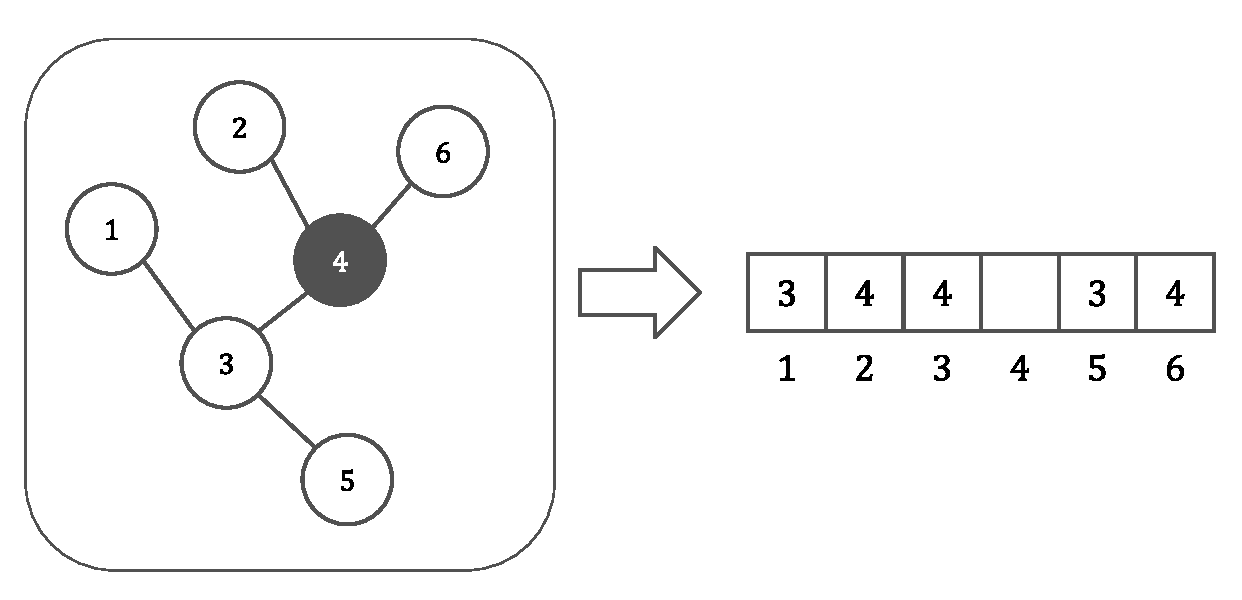
\includegraphics[scale=0.6]{figures/graphs1.pdf}
  \caption{Exemplo de representação implícita de árvores, com vértice raiz realçado}
  \label{fig:graphs1}
\end{figure}

Esta \emph{eficiência} do teste de adjacência parece estar ligada ao fato da representação manter um número limitado de bits para cada vértice e utilizar apenas estes bits para o teste. Assim, podemos definir, motivados por essa intuição, o conceito de representação implícita \footnote{Na literatura é usual definir como representação implícita apenas aquelas com $f(n) = n \log n$. A definição que apresentamos aqui é uma versão generalizada, formalizada em \cite{spinrad2003efficient}, que é mais apropriada para os problemas que trataremos a frente.} como a seguir. Seja $C$ uma classe de grafos com $2^{\Theta(f(n))}$ elementos. Uma representação $R$ de um grafo $G \in C$, de $n$ vértices é dita implícita se:
\begin{enumerate}  
\item \emph{ela é assintoticamente ótima:} a representação requer apenas $O(f(n))$ bits no total;
\item \emph{ela distribui informação entre os vértices:} a parcela de representação correspondente a cada vértice possui apenas $O(f(n)/n)$ bits;
\item \emph{o teste de adjacência é local:} para testar a adjacência entre dois vértices, apenas as informações locais a eles são necessárias.
\end{enumerate}

Um exemplo de classe que respeita essas propriedades são os \emph{grafos de intervalo}. Um grafo é dito de intervalo se cada um de seus vértices puder ser mapeado para um intervalo na reta real, de modo que há aresta entre dois vértices se e somente se os respectivos intervalos possuem interseção não-vazia. Esta classe possui grande utilidade prática e pode ser definida uma representação implícita simples baseada na definição da classe. A representação consiste em enumerar as extremidades dos intervalos, na ordem em que aparecem na reta real, com inteiros no intervalo $[1;2n]$. Representa-se cada vértice do grafo com os dois inteiros correspondentes às extremidades de seu respectivo intervalo. Um exemplo pode ser visto na Figura~\ref{fig:graphs2}. Dois vértices serão considerados adjacentes se e somente se os intervalos representados pelos inteiros possuírem interseção não-vazia, o que pode ser testado em tempo constante. Apenas $\Theta(\log n)$ bits são usados para representar cada vértice e $\Theta(n\log n)$ bits são usados para representar o grafo inteiro. Isto indica que há $2^{O(n \log n)}$ grafos de intervalo possíveis.

\begin{figure}[!htbp]
  \centering
  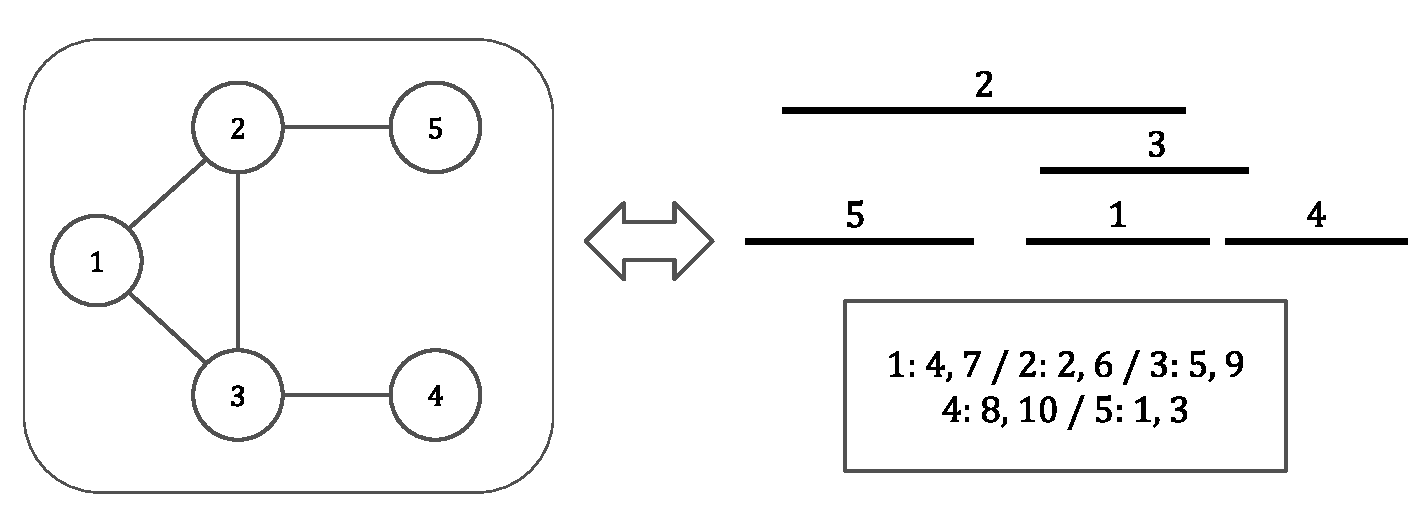
\includegraphics[scale=0.6]{figures/graphs2.pdf}
  \caption{Exemplo de representação implícita de grafos de intervalo}
  \label{fig:graphs2}
\end{figure}


Para verificar o limite inferior no número de elementos na classe, considere grafos com $n$ vértices onde cada um dos $n/2$ primeiros vértices possuem uma aresta para um vértice distinto entre os $n/2$ últimos. Esta é uma subclasse dos grafos de intervalo. Por definição, ela possui $(n/2)!$ possíveis grafos com $n$ vértices. Como, $(n/2)!$ é $2^{\Theta(n \log n)}$, segue que há $2^{\Theta(n \log n)}$ grafos de intervalo e, portanto, a representação apresentada anteriormente é ótima.

Encontrar uma representação que respeite as propriedades necessárias pode não ser trivial. De fato, para muitas classes pode ser que não exista representação implícita. Por exemplo, considere a classe de grafos onde $m = O(n)$. Usando uma lista de adjacência, é possível representar grafos nesta classe usando $O(n \log n)$ bits, o que indica que esta classe possui $2^{O(n\log n)}$ elementos. É impossível, entretanto, satisfazer as propriedades (2) e (3) simultaneamente, pois é possível transformar um grafo $G$ qualquer para um $H$ nesta classe introduzindo $n^2$ vértices de grau zero. Assim, se houvesse uma representação implícita para $H$, seria possível representar os $G$ usando apenas $O(n \log n)$ bits. Isto implicaria que é possível representar qualquer grafo usando $O(n \log n)$ bits, o que é absurdo.

A possibilidade de construir grafos em classes com $2^{\Theta(n\log n)}$ grafos a partir de grafos gerais apenas adicionando vértices pode posar como um desafio para definir propriedades gerais sobre essas classes. Por isso, utiliza-se mais frequentemente classes hereditárias na busca por classes com representações implícitas. Uma classe é dita \emph{hereditária} se para todo grafo $G$ nesta classe, todo subgrafo induzido de $G$ também está na classe. A classe definida anteriormente (onde $m = O(n)$) não é hereditária, pois a remoção de vértices de grafos naquela classe pode resultar em grafos fora dela. É possível provar que uma classe hereditária $C$ contém $2^{\Theta(n^2)}$ se e somente se ela contém todos os grafos bipartidos, todos os co-bipartidos ou todos os grafos \emph{split}. É uma conjectura aberta se toda classe hereditária com $2^{O(n \log n)}$ grafos possui uma representação implícita, é conhecida como \emph{Conjectura da Representação Implícita} \cite{kannan1992implicat,spinrad2003efficient,chandoo2016implicit}. É importante notar que mesmo classes não-hereditárias podem possuir representação implícita (por exemplo, árvores).

A fim de estudar o uso de estruturas de dados probabilísticas no problema de representações eficientes de grafos, introduzimos aqui a definição de \emph{representação probabilística} como uma representação que relaxa o teste de adjacência, permitindo uma taxa fixa de falsos positivos e falsos negativos independente do tamanho do grafo (uma taxa de erro zero significa que a representação é em particular determinística).

Definimos ainda a ideia de representação implícita probabilística, que estende a definição apresentada anteriormente para permitir a aplicação representações probabilísticas. Logo, uma representação é implícita probabilística se ela respeitar as três propriedades de representações implícitas admitindo o uso de uma representação probabilística.

\section{Representações probabilísticas: uma aplicação}\label{sec:graphs:example}

Como visto na seção anterior, não é possível representar deterministicamente uma classe com $2^{\Theta(f(n))}$ grafos de $n$ vértices usando $o(f(n))$ bits. Entretanto, há situações onde este limite pode não ser viável na prática ou, mesmo sendo viável, necessite de estruturas especiais para alcançar um uso de recursos aceitável.

Como exemplo motivador, analisaremos o problema da montagem de fragmentos de DNA sequenciados através do método \emph{shotgun}. Neste método, são sequenciadas somente cadeias curtas (entre cem e mil pares de bases). Cadeias mais longas são subdividas em fragmentos, que precisam ser remontados posteriormente. A Figura~\ref{fig:graph_dna_assembly} exemplifica o processo.

\begin{figure}[!htbp]
  \centering
  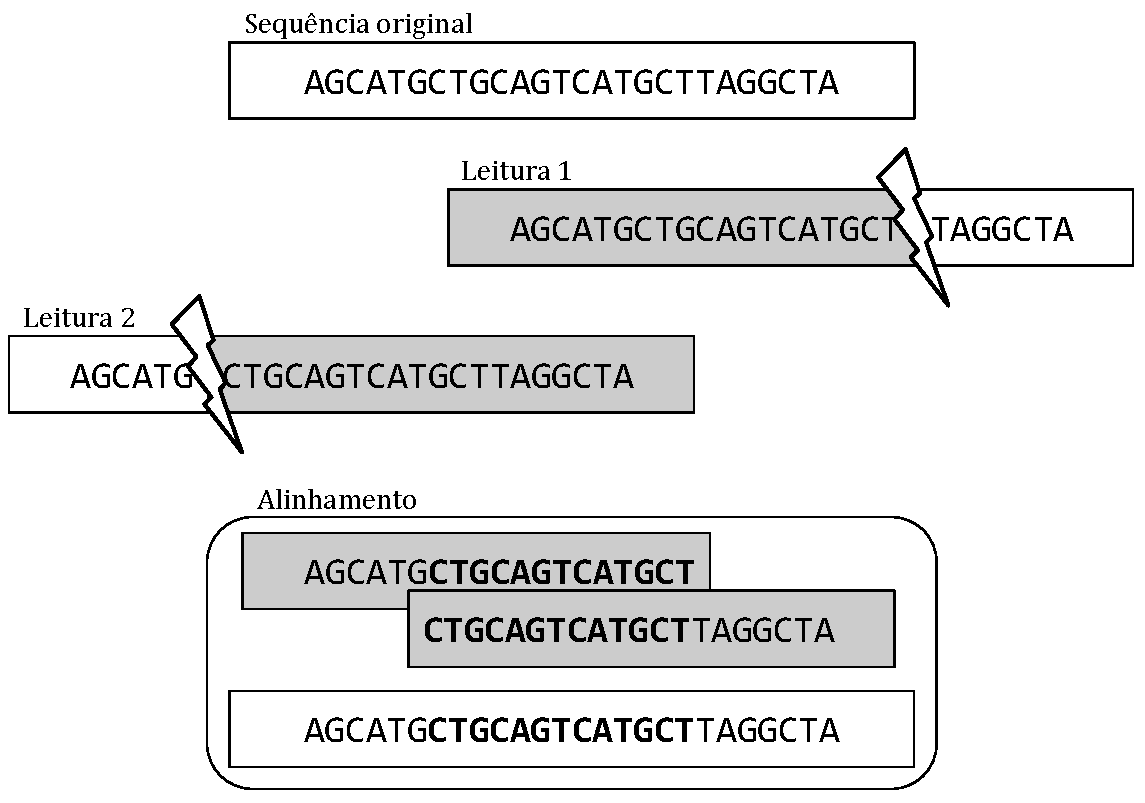
\includegraphics[scale=0.6]{figures/graph_dna_assembly.pdf}
  \caption{Processo de remontagem de sequências a partir de fragmentos}
  \label{fig:graph_dna_assembly}
\end{figure}

Este tipo de sequenciamento é essencial para o entendimento da composição microbial de amostras obtidas diretamente do ambiente (metagenômicas) que, em conjunto, desempenham importante papel no equilíbrio bioquímico de seu ambiente de origem. Mas, para permitir uma remontagem com alto grau de confiança, é preciso realizar, armazenar e processar um número muito grande de leituras. Somente recentemente o equipamento necessário para realizar estas leituras começou a tornar-se acessível. Entretanto, os algoritmos tradicionais para a remontagem dos fragmentos não lidam satisfatoriamente com o imenso volume de dados gerados no processo.

Para fins de processamento, as leituras são decompostas em palavras de um certo tamanho fixo $k$ -- chamadas de $k$-mers -- e organizadas como um grafo \emph{de Bruijn} \cite{pevzner2001eulerian,compeau2011apply}, onde cada vértice representa um $k$-mer e há aresta entre dois vértices se os $k$-mers relativos a eles compartilham $k-1$ bases contíguas em alguma leitura. A Figura~\ref{fig:graph_dna_bruijn} mostra um exemplo desta construção. 

\begin{figure}[!htbp]
  \centering
  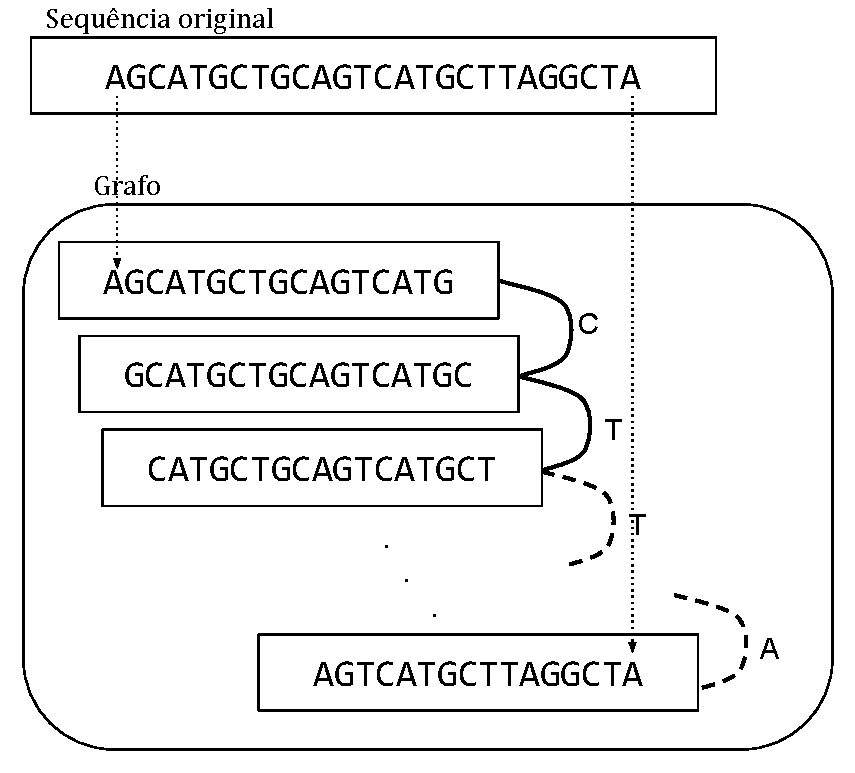
\includegraphics[scale=0.6]{figures/graph_dna_bruijn.pdf}
  \caption{Grafo \emph{de Bruijn} gerado a partir de 16-mers de uma única sequência}
  \label{fig:graph_dna_bruijn}
\end{figure}

É possível perceber que, nesse grafo, cada vértice pode ter no máximo oito arestas, uma para cada base possível (G, T, C e A) em cada uma das extremidades do $k$-mer. Espera-se também que a maioria dos vértices tenha duas arestas. Além disso, a escolha de $k$ define o número máximo de vértices do grafo, dado por $4^k$. Isto influencia também a probabilidade de encontrar arestas espúrias (que não representam um trecho real de sequência genômica).

O processo de montagem consiste em encontrar um caminho Hamiltoniano neste grafo. Em \cite{pevzner2001eulerian} é mostrada uma construção alternativa que permite efetuar a montagem através da busca por um caminho Euleriano.

Para amostras de um mesmo indivíduo, os métodos tradicionais ainda conseguem representar e processar os dados utilizando \emph{hardware} amplamente disponível. Gnerre et al. \cite{gnerre2011high} mostram que é possível realizar a montagem de DNA humano, a partir de cerca de $3 \times 10^9$ leituras, utilizando 512GB de RAM. Este custo é bastante viável, especialmente considerando os recursos computacionais de provedores comerciais de serviços de nuvem. Entretanto, para amostras metagenômicas complexas, muitos terabytes de memória seriam necessários para representar todas as sequências de diferentes espécies em um mesmo grafo. Como essas leituras representam múltiplos espécimes de espécies diferentes, a fim de diminuir o custo de processamento total, pode-se empregar uma técnica de particionamento, onda usa-se algum método menos custoso para dividir esse grafo em componentes (para cada espécie ou grupo de indivíduos) que podem ser processados separadamente em momentos diferentes.

Em \cite{pell2012scaling}, os autores relatam o uso de filtros de Bloom para representar probabilisticamente o grafo inteiro, podendo, dependendo da configuração de falsos positivos, utilizar apenas 4 bits para representar cada $k$-mer. Esta representação é utilizada para percorrer o grafo identificando seus componentes e realizando o particionamento das leituras. A vantagem do Filtro de Bloom neste caso é a impossibilidade de falsos negativos, que, se possíveis, poderiam particionar leituras de um mesmo espécime em componentes diferentes.

Na construção sugerida, as arestas não são armazenadas, apenas os vértices. Qualquer par de vértices cujos $k$-mers compartilhem $k-1$ bases contíguas são considerados adjacentes. O passo de uma busca no grafo consiste em partir de um certo $k$-mer e verificar a existência de todos os oito possíveis $k$-mers adjacentes em todo o grafo. Desta forma, o problema de representação é reduzido à representação probabilística do teste de pertinência no conjunto de $k$-mers. O Filtro de Bloom é diretamente aplicável neste caso.

O argumento defendido pelos autores é que, em dados reais, a taxa de falsos positivos tende com maior probabilidade a causar uma elaboração local nos componentes, em vez de causar conexões espúrias entre componentes. Argumenta-se também que através de análise experimental, probabilidades de falso positivo até cerca de 18\% não costumam realizar mudanças significativas na macroestrutura do grafo. Assim, definindo um valor de $q = 4$ bits por elemento no Filtro de Bloom, é possível alcançar uma taxa de falsos positivos de cerca de 15\%, que é suficiente para o processo de particionamento das amostras metagenômicas.


\section{Filtro de Bloom como representação implícita}\label{sec:graphs:bloom}

Os resultados em \cite{pell2012scaling} suscitam a discussão sobre a viabilidade de representações probabilísticas para outras classes de grafos além dos \emph{de Bruijn}.

Como exemplo, podemos estudar o uso direto de filtros de Bloom para representação do conjunto de arestas $E$ em grafos gerais. Como o objetivo é representar grafos gerais, o desejável é que seja possível construir o filtro com complexidade de espaço igual a $\Theta(n^2)$, porém com um menor fator constante.

A ideia consiste em encontrar uma função \emph{hash} $h: E \to [1..m_B]$, que mapeia arestas do grafo em posições em um filtro de Bloom de $m_B$ bits. De fato, filtros de Bloom permitem representar toda a adjacência do grafo utilizando 10 bits por aresta -- isto é, O(m) bits --, a fim de alcançar uma probabilidade de falsos positivos menor que 1\%. Esta representação mostra grande valor para representação de grafos esparsos, apesar de ser igualmente eficiente à matriz de adjacência ao requerer $\Theta(n^2)$ bits para representar o grafo no pior caso (ex.: grafos completos).

Esta representação possui uma característica importante: toda aresta do grafo é representada deterministicamente. Isto é, se a aresta existe no grafo original, com 100\% de probabilidade ela existirá na versão probabilística. Desta propriedade, segue que se um teste de adjacência na representação probabilística resultar em resposta negativa, é garantido que a aresta não exista no grafo original. Isto é, como característica do filtro de Bloom, não há falsos negativos. O contrário, entretanto, não é verdade. Em testes de adjacência entre vértices não-adjacentes, há probabilidade de falsos positivos. Isto significa, que para uma probabilidade de falsos positivos $p$, espera-se encontrar $p(\frac{n(n-1)}{2}-m)$ arestas na representação probabilística que não existem no grafo original.

É importante notar que, construída da forma apresentada, esta não seria uma representação implícita, mesmo se relaxarmos o requisito do teste de adjacência para permitir respostas probabilísticas. Isto se deve a esta representação não distribuir a informação entre os vértices. De fato, não há representação local nos vértices.

Uma variação que resolveria este problema seria manter um filtro de Bloom para cada vértice. Assim, para cada vértice $v$, teríamos um filtro de Bloom com $10 \times \text{d}(v)$ bits -- onde $\text{d}(v)$ é o grau do vértice -- de forma que a probabilidade de falsos positivos em cada um deles é exatamente igual e equivalente à versão anteriormente apresentada. Assim, para cada vértice, esta representação necessita de $O(\text{d}(v))$ bits que, no pior caso, é equivalente a uma linha da matriz de adjacência ($O(n)$ bits), entretanto, permite representação de grafos esparsos com complexidade menor que a lista associada a cada vértice numa lista de adjacência, que requer $O(\text{d}(v) \log n)$ bits.

A Figura~\ref{fig:graph:bloom} compara os resultados empíricos para sucessivos testes em grafos aleatórios com $n = 100$ e $m$ variando em todos os valores possíveis para um grafo com este tamanho. Ambas as variantes apresentadas nesta seção foram testadas. Note que para $m=0$, por característica da construção filtro de Bloom, não há arestas espúrias.

\begin{figure}[!htbp]
\centering
\scalebox{0.80}{\begin{tikzpicture}[
        declare function = {
            p(\n,\m) = 0.008193722*(\n*(\n-1)/2-\m);
        }
    ]
	\begin{axis}[
	    title=Filtro de Bloom único,
	    scaled ticks=false, 
        grid=both,
        ylabel={arestas espúrias},
    	xlabel=número de arestas ($m$),
        xmin=0, xmax=5000,
        ymin=0, ymax=50,
		legend columns=1, 
	    legend style={legend pos=outer north east,}
    ]

	\addplot[line width=1pt, mark=*,black,smooth, mark options={scale=0.75}] table[x=m,y=v1] {files/graph_bloom.txt};
	\addplot[smooth, mark options={scale=0.75}, line width=5pt,color={rgb:black,1;white,1},opacity=0.4] table[x=m,y=e] {files/graph_bloom.txt};
    %\addplot[dotted, line width=1pt, mark=none,black,smooth] table[x=k,y=max] {files/minhash_shakespeare.txt};
	%\legend{esperado,shakespeare, $\pm 1 \sigma$, min/max };


	\end{axis}
\end{tikzpicture} \begin{tikzpicture}[
        declare function = {
            p(\n,\m) = 0.008193*(\n*(\n-1)/2-\m);
        }
    ]
	\begin{axis}[
	    title=Um fitro de Bloom para cada vértice,
	    scaled ticks=false, 
        grid=both,
        xmin=0, xmax=5000,
        ymin=0, ymax=50,
		xlabel=número de arestas ($m$),
		yticklabel={\ },
		legend columns=1, 
	    %legend style={legend pos=outer north east,}
    ]

	\addplot[line width=1pt, mark=*,black,smooth, mark options={scale=0.75}] table[x=m,y=v2] {files/graph_bloom.txt};
	\addplot[smooth, mark options={scale=0.75}, line width=5pt,color={rgb:black,1;white,1},opacity=0.4] table[x=m,y=e] {files/graph_bloom.txt};
    %\addplot[dotted, line width=1pt, mark=none,black,smooth] table[x=k,y=max] {files/minhash_shakespeare2.txt};
	\legend{observado, esperado};

	\end{axis}
\end{tikzpicture}}
\caption{Arestas espúras em um grafo com $n=100$.}
\label{fig:graph:bloom}
\end{figure}

\section{\emph{MinHash} como representação implícita}\label{sec:graphs:countmin}

Uma propriedade desejável de representações probabilísticas é que elas sejam capazes de representar grafos utilizando menos recursos que as melhores representações determinísticas. Nesta seção, apresentaremos algumas ideias de construções baseadas em funções \emph{hash} sensíveis a localidade, em especial \emph{MinHash} e \emph{SimHash}, apresentadas anteriormente na Seção~\ref{sec:minhash}.

Essas estruturas funcionam sumarizando conjuntos através de assinaturas compactas que permitem, em tempo logarítmico ou menor, estimar um índice de semelhança entre os conjuntos que representam. No caso de \emph{MinHash}, este índice é o coeficiente de \emph{Jaccard} $J(A, B) = \frac{|A \cap B|}{|A \cup B|}$. No caso do \emph{SimHash}, o índice é relativo à similaridade de cosseno dos vetores que representam os conjuntos $S(A, B) = 1 - \arccos \left( \frac{|A \cap B|}{\sqrt{|A| \cdot |B|}}\right)/\pi$. Todos os métodos nesta seção podem ser usados com ambas as estruturas, porém, por brevidade, referenciaremos apenas \emph{MinHash} ao longo do texto.

A ideia principal que trabalharemos nesta seção consiste em representar cada vértice como um conjunto, de forma que seja possível verificar a adjacência entre dois vértices comparando a semelhança entre os conjuntos que os representam. Isto é, dada uma família de conjuntos $\{S_1, \ldots, S_n\}$ e uma métrica de similaridade $f(S_i, S_j) \to \mathbb{R}$, e um limite inferior $\delta$, definimos o grafo como $(V = \{v_1, \ldots, v_n\}, E = \{(v_i, v_j) : 1 \leq i < j \leq n | f(S_i, S_j) > \delta\})$. Um problema que abordaremos adiante será o de como escolher tais conjuntos que representam um grafo. De antemão, porém, observamos que não é necessário que escolhamos uma família de conjuntos ótima no sentido de minimizar cardinalidade dos mesmos ou de sua união, por exemplo, pois os conjuntos em si não serão armazenados, somente suas assinaturas \emph{MinHash}. Desta forma é possível estimar a adjacência entre dois vértices através da estimativa de similaridade entre seus conjuntos. 

A vantagem desta abordagem vem das propriedades de \emph{MinHash}. O erro relativo da estimativa de similaridade cresce em fator sublinear ao tamanho do conjunto, sendo mais significativa a quantidade de elementos na assinatura. Desta, forma, mesmo que o processo de construção dos conjuntos envolva a criação de conjuntos com cardinalidades polinomiais sobre o número de vértices do grafo, a assinatura \emph{MinHash} que precisará ser armazenada para cada vértice irá conter apenas um número constante de elementos. 

\subsection{Generalizando grafos de interseção}

A ideia de representar a adjacência de vértices em um grafo através de conjuntos remete diretamente a ideia de grafos de interseção. Um grafo de interseção de $n$ vértices é definido através de uma família de conjuntos $\{S_1, \ldots, S_n\}$, de forma que há adjacência entre $v_i$ e $v_j$ se e somente se $S_i \cap S_j \neq \varnothing$. Usando notação apresentada anteriormente, é possível definir também através da função de similaridade $f(S_i, S_j) = J(S_i, S_j) = \frac{|A \cap B|}{|A \cup B|}$ e $\delta = 0$.

É fácil observar que todo grafo é um grafo de interseção. Por exemplo, é possível definir $S_i$ como o conjunto de todas as arestas incidentes em $v_i$. Assim, a interseção $S_i \cap S_j$ irá conter uma aresta se e somente se $v_i$ e $v_j$ compartilharem uma aresta. A Figura~\ref{fig:graph_intersection} demonstra esta construção.

\begin{figure}[!htbp]
  \centering
  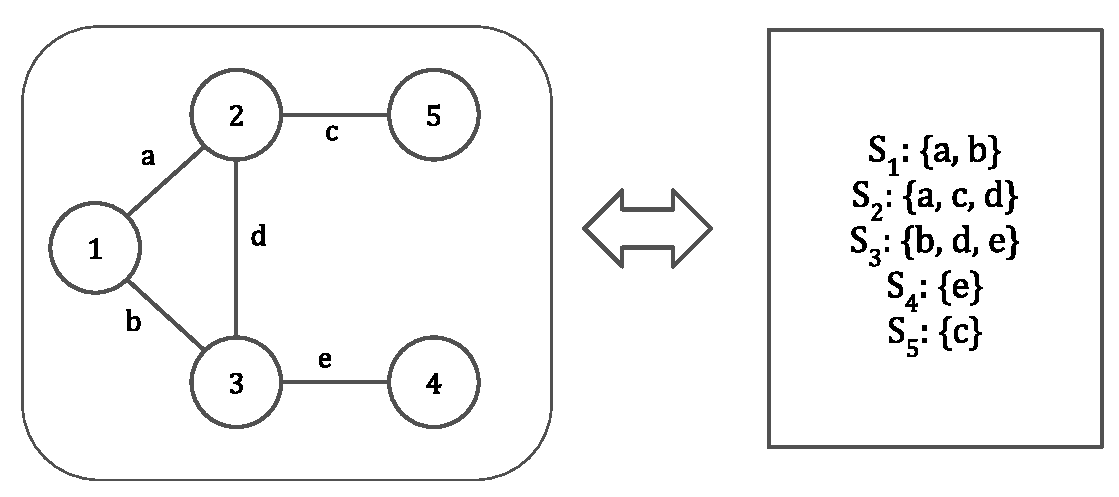
\includegraphics[scale=0.6]{figures/graphs_intersection.pdf}
  \caption{Exemplo de grafos de interseção}
  \label{fig:graph_intersection}
\end{figure}

Apresentamos aqui uma construção generalizada para outros valores de $\delta$, em especial, para qualquer $\delta \in \mathbb{Q} \cap [0;1]$. Dado um grafo $G = (V, E)$ qualquer, $\delta = \frac{x}{y}$, o objetivo é construir conjuntos $\{S_1, \ldots, S_n\}$ tais que $(v_i, v_j) \in E$ se e somente se $J(S_i, S_j) > \delta$.

Para exemplificar a construção, começamos descrevendo um grafo com $E = \varnothing$. Neste grafo, todos os conjuntos são construídos para ter $J(S_i, S_j) = \delta$, ou seja, representando uma não-adjacência. Para tanto, cada conjunto é composto por $a$ elementos comuns entre os conjuntos e $b$ elementos únicos de cada conjunto. Desta forma, $|S_i \cap S_j| = a$ e $|S_i \cup S_j| = a + 2b$. Então, é possível determinar a proporção de $a$ e $b$ exata pela equação:
\[
    \frac{a}{a+2b} = \delta = \frac{x}{y} \Rightarrow a = \frac{2x}{y-x}b
\]

Por esta relação, percebe-se que é suficiente escolher $b$ de forma que seja divisível por $y-x$. Para modelar as adjacências, no conjunto de cada vértice $v$ substitui-se $\deg(v)$ dos $b$ elementos únicos em cada conjunto pelas arestas incidentes no vértice relativo aquele conjunto. Portanto, também é preciso escolher $b \geq \Delta(G)$, onde $\Delta(G)$ é o maior grau de um vértice em $G$.

Por exemplo, para $\delta = \frac{1}{2}$, temos que $a = 2b$. A Figura~\ref{fig:graph_intersection2} mostra um exemplo prático. Na figura, uma posição de elemento sem identificador significa que podemos escolher um elemento distinto qualquer. No exemplo, como $\Delta(G) = 3$, podemos assumir $b = 3$ e $a = 6$, logo, qualquer não-adjacência possui $J(S_1, S_2) = \frac{1}{2}$ e as adjacências possuem $J(S_1, S_2) = \frac{7}{12} > \frac{1}{2}$.

\begin{figure}[!htbp]
  \centering
  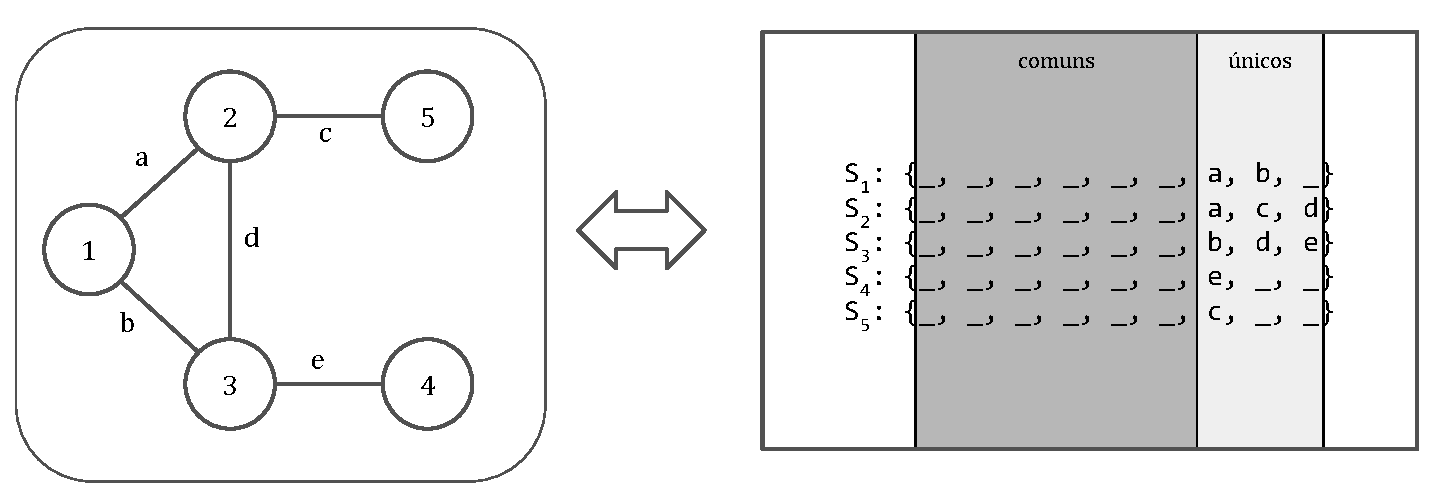
\includegraphics[scale=0.6]{figures/graphs_intersection2.pdf}
  \caption{Exemplo de grafos de interseção para $\delta = 0,5$}
  \label{fig:graph_intersection2}
\end{figure}

De uma forma geral, a diferença entre os índices de similaridade que denotam adjacência e não-adjacência será igual a $(a + 2b)^{-1}$. Dado que $b \geq \Delta(G) $, essa diferença tende a tornar-se desprezível conforme o grafo cresce, se $\Delta(G) = \omega(1)$. Caso contrário, ela fica constante. Exemplos deste último caso estão grafos com grau limitado, como o caso dos grafos k-regulares (para k fixo) e os grafos de Bruijn para k-mers com k-fixo. Isto torna o uso desta construção com \emph{MinHash} inviável para representar grafos de forma probabilística no caso geral, pois com o erro associado à estimativa, a incerteza sobre a adjacência ou não de dois vértices tornará o teste em grafos muito grandes indistinguível de uma resposta arbitrária.

Por este motivo, nas próximas seções, buscaremos apresentar construções que garantam um certo intervalo entre similaridades que representam adjacências e não-adjacências. Mais específicamente:
\[
    (v_i, v_j) \notin E \leftrightarrow f(S_i, S_j) \leq \delta_A
\]\[
    (v_i, v_j) \in E \leftrightarrow f(S_i, S_j) \geq \delta_B
\]

Embora esteja claro que para $\delta_A = \delta$ e $\delta_B = \delta + \epsilon$ (onde $\epsilon$ é um valor tão pequeno quanto necessário) existe construção viável para grafos gerais, como recém demonstrado, ainda é um problema aberto se para valores arbitrários de $\delta_A$ e $\delta_B$ esta construção sempre existe. Por exemplo, provaremos na Seção~\ref{sec:graphs:bipartite} que para $\delta_A = 0,4$ e $\delta_B = 0,6$, não há tal construção para grafos bipartidos. Por isso, abordaremos progressivamente o assunto para classes específicas de grafos de forma a explorar melhor as propriedades do problema.

\subsection{Construção para árvores}

Nesta seção, mostramos que é possível construir uma representação probabilística para árvores com complexidade de espaço menor do que a melhor construção determinística para  $\delta_A = \frac{1}{3}$ e $\delta_B = \frac{1}{2}$. Esta construção é recursiva e baseia-se na ideia de que subconjuntos $S \subset U$, tais que $2|S| = |U|$, possuem índice de Jaccard $J(S, U) = \frac{1}{2}$. Então, partindo de um vértice arbitrário como raiz da árvore (portanto transformando a árvore em enraizada) com um conjunto inicial qualquer, define-se um procedimento para a escolha de subconjuntos de forma que, para dois filhos $a$ e $b$ quaisquer, seus subconjuntos $S_a$ e $S_b$, respectivamente, respeitem $J(S_a, S_b) \leq \frac{1}{3}$. Os filhos desses vértices, por sua vez, podem ter conjuntos definidos pela extensão dos conjuntos de seus pais. A partir daí, o processo torna-se recursivo. A Figura~\ref{fig:graph_tree_ex1} mostra um exemplo desta construção usando conjuntos de números inteiros.

\begin{figure}[!htbp]
  \centering
  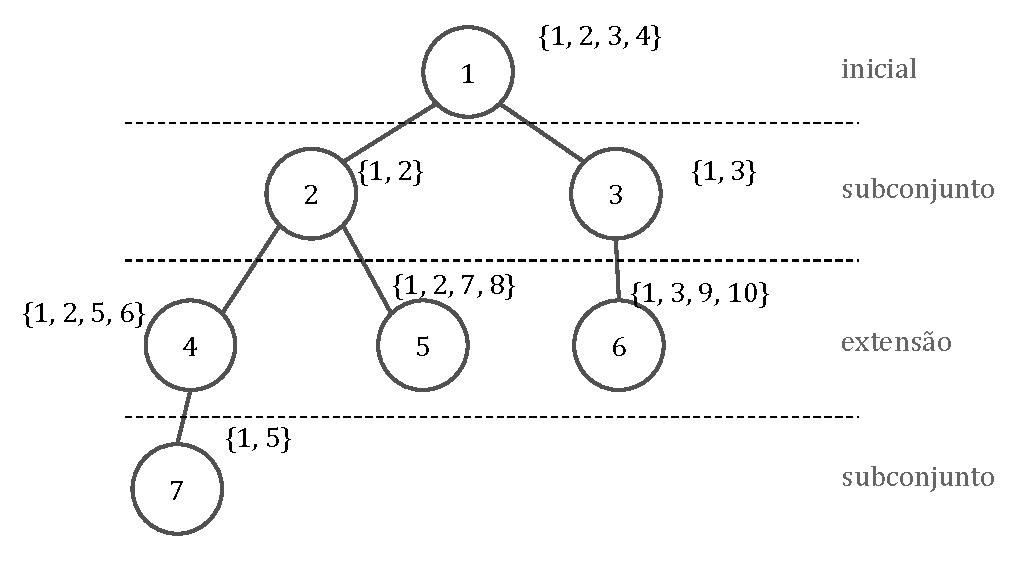
\includegraphics[scale=0.6]{figures/graphs_tree_ex1.pdf}
  \caption{Exemplo de construção de conjuntos para uma árvore}
  \label{fig:graph_tree_ex1}
\end{figure}

O número de elementos no conjunto inicial deve ser um valor $x$ suficiente para que seja possível extrair até $\Delta(G)$ subconjuntos de $x/2$ elementos, de forma que nenhum par $(S_a, S_b)$ de subconjuntos possua $J(S_a, S_b) > \frac{1}{3}$. Além disso, nunca devem ser escolhidos mais do que $x/4$ elementos do conjunto que tenham sido originados de um vértice avô, para garantir que o índice de Jaccard entre vértices e seus avôs seja sempre menor que $\frac{1}{3}$.

Qualquer estratégia de seleção de subconjuntos que tenha essas propriedades poderia ser usada. Oferecemos, como exemplo, uma estratégia capaz de selecionar, a partir de um conjunto com $x$ elementos, $x/2$ subconjuntos de $x/2$ elementos, tais que quaisquer dois subconjuntos $S_a, S_b$ possuam exatamente $x/4$ elementos em comum, ou seja, $J(S_a, S_b) = \frac{x/4}{3x/4} = \frac{1}{3}$.

A ideia desta estratégia é gerar uma cadeia binária $s$, com $|s|=x/2$ que represente a seleção de elementos $S \subset \{a_1,\ldots,a_x\}$ de modo que se o $i$-ésimo bit de $s$ tem o valor $b$, então $a_{2i-1+b}$ pertence a S, como exemplificado a partir de um conjunto com oito elementos, na Figura~\ref{fig:graph_tree_bintable}.

\begin{figure}[!htbp]
  \centering
  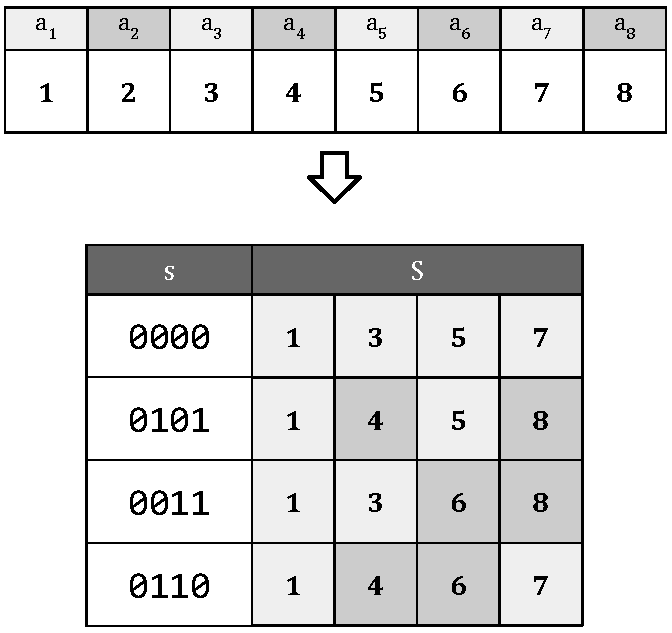
\includegraphics[scale=0.6]{figures/graphs_tree_bintable.pdf}
  \caption{Exemplo de subconjuntos para um conjunto inicial com oito elementos}
  \label{fig:graph_tree_bintable}
\end{figure}

A geração das cadeias binárias pode ser feita através de uma construção iterativa. Onde partindo de uma matriz $1\times1$, a cada passo a matriz é quadruplicada, sendo o quadrante inferior direito invertido, como exemplifica a Figura~\ref{fig:graph_tree_binbuild}.

\begin{figure}[!htbp]
  \centering
  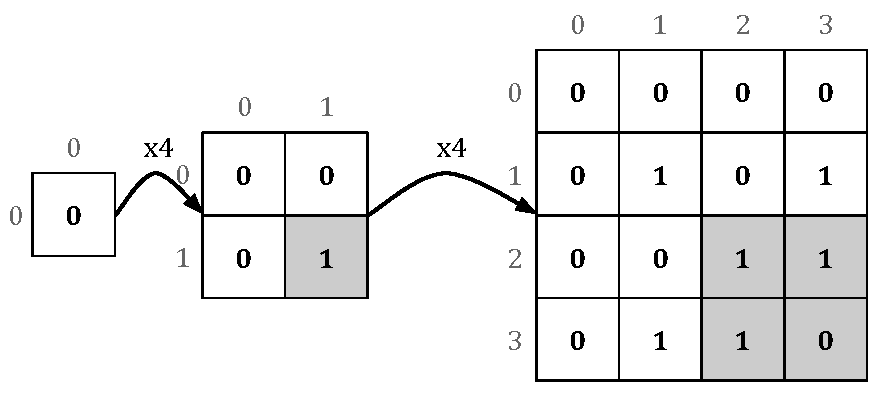
\includegraphics[scale=0.6]{figures/graphs_tree_binbuild.pdf}
  \caption{Processo de construção de cadeias binárias}
  \label{fig:graph_tree_binbuild}
\end{figure}

Esta construção garante que a cada passo o número de linhas duplique, mas cada linha seja distinta das demais e possua exatamente metade de seus bits em comum com qualquer outra linha. Uma construção mais simples desta tabela vale-se do fato de que qualquer célula $(i, j)$ nesta tabela é igual ao resto da divisão do número de bits 1 em \texttt{i\&j} por dois, onde \texttt{\&} denota o operador binário aplicado bit-a-bit.

Baseado nesta construção, podemos definir o algoritmo que gera os conjuntos para cada vértice do grafo. Ele pode ser visto no Algoritmo~\ref{alg:graphs:treemain}.

\begin{algorithm}
\linespread{1}\selectfont
\caption{Gera os conjuntos $S_v$ para cada vértice $v$ em uma árvore $G$}
\label{alg:graphs:treemain}
\begin{algorithmic}[1]
\State{seja $\Delta(G)$ o maior grau de um vértice em $G$}
\State{seja $q = 2^{\lceil \log_2(d_{max}(G)) \rceil+1}$}
\State{seja $\rho(v, n)$ uma função que retorna $n$ elementos únicos ao vértice $v$}

\Function{GeraSubconjunto}{$S = \{s_0, s_2, \cdots, s_{q-1}\}$, $i$}
    \State{$R \gets \varnothing$}
    \For{$j \in [0, q/2)$}
        \State{$x \gets \Call{BitCount}{\texttt{i\&j}}\%2$}     
        \State{$R \gets R \cup s_{2j+x}$}
    \EndFor
    \Return{R}
\EndFunction

\Procedure{VisitaFilhos}{$G, v$}
    \State{marcar $v$ como visitado}

    \State{$i \gets 0$}
    
    \For{\text{cada} vizinho não-visitado $u$ de $v$ em $G$}
    
        \If{$|S_v| = q$}
            \State{definir $S_u = \Call{Gera-Subconjunto}{S_v, i}$}
            \State{$i \gets i + 1$}
        \Else
            \State{definir $S_u = S_v \cup \rho(u, q/2)$}
        \EndIf
        \State{\Call{VisitaFilhos}{$G, u$}}
    \EndFor
\EndProcedure

\Procedure{GeraConjuntos}{$G$}
    \State{$v \gets$ um vértice qualquer em $G$}
    \State{definir $S_v = \rho(r, q)$}
    \State{\Call{GeraFilhos}{G, r}}
\EndProcedure
\end{algorithmic}
\end{algorithm}

Esta técnica permite representar probabilisticamente o grafo através de assinaturas com número constante de bits, alcançando uma representação probabilística com $O(n)$ bits (na versão com \emph{SimHash}) para uma classe com $2^{O(n log n)}$ grafos de $n$ vértices. Portanto, esta representação possui complexidade de espaço menor do que a representação ótima da classe. Na prática, entretanto, para árvores com até cerca de $2^{64}$ vértices, a representação determinística continua sendo mais eficiente (por possuir um fator constante menor).

Para verificar a eficácia desta técnica de construção na prática, foram realizados experimentos com árvores aleatórias, variando alguns parâmetros, e as respectivas taxas de falsos positivos e falsos negativos foram registradas.

Considera-se falso negativo quando uma aresta é erroneamente representada como uma não-aresta, e falso positivo são o caso inverso, quando uma não-aresta é representada como uma aresta. Nos testes, ambos estão representados em valores relativos. A taxa de falsos positivos é a razão entre o número de falsos positivos e a quantidade de não-arestas no grafo. E vice-versa. Em tese, é possível ter tanto a taxa de falsos positivos como de falsos negativos iguais a 100\%, mas isso não ocorre no teste em momento algum.

Tratando-se de uma árvore, um grafo esparso, os falsos negativos geralmente são menos desejáveis do que falsos positivos, mas de fato qual dos dois é mais ou menos aceitável depende da aplicação. A construção que apresentamos nesta seção gera uma representação \emph{MinHash} com $\delta_A = \frac{1}{3}$ e $\delta_B = \frac{1}{2}$. O valor da similaridade computada, entretanto, pode estar entre $\delta_A$ e $\delta_B$ devido ao erro associado à estrutura probabilística. Portanto, a verificação de adjacência nesta representação depende da escolha de um limite após o qual os valores de similaridades passam a ser considerados arestas.

O primeiro teste analisa este limite, que por analogia também chamaremos de $\delta$. Isto é, dois vértices $v_i$ e $v_j$ são considerados adjacentes se, dada a função probabilística de similaridade $f$, $f(S_i, S_j) > \delta$. No teste, variamos os valores de $\delta$, com árvores aleatórias de 200 vértices, para $k=64$ e $k=128$ e observamos as curvas geradas pelas taxas de falsos positivos e falsos negativos. O resultado pode ser visto na Figura~\ref{fig:graph:delta}.


\begin{figure}[!htbp]
\centering
\scalebox{0.80}{

\begin{tikzpicture}[]
	\begin{axis}[
	    title={MinHash ($k=64$)},
	    grid=both,
		yticklabel=\pgfmathparse{100*\tick}\pgfmathprintnumber{\pgfmathresult}\,\%,
        ylabel={percentual},
		xlabel=limite de teste ($\delta$),
        xmin=0, xmax=1,
        ymin=0, ymax=1,
    ]

	\addplot[black,stack plots=y,area style,fill=black!50] table[x=delta,y=p1] {files/graphs_delta.txt} \closedcycle;
	\addplot[black,stack plots=y,area style,fill=black!20] table[x=delta,y=n1] {files/graphs_delta.txt} \closedcycle;
	\addplot[dashed, black] coordinates{(0.416666667,0) (0.416666667,1)};

	\end{axis}
\end{tikzpicture} \begin{tikzpicture}[
        declare function = {
            p(\n,\m) = 0.008193*(\n*(\n-1)/2-\m);
        }
    ]
	\begin{axis}[
	    title={SimHash ($k=64$)},
	    scaled ticks=false, 
        grid=both,
        xmin=0, xmax=1,
        ymin=0, ymax=1,
		xlabel=limite de teste ($\delta$),
		yticklabel={\ },
		legend columns=1, 
        %legend style={legend pos=outer north east,}
    ]

	\addplot[black,stack plots=y,area style,fill=black!50] table[x=delta,y=p2] {files/graphs_delta.txt} \closedcycle;
	\addplot[black,stack plots=y,area style,fill=black!20] table[x=delta,y=n2] {files/graphs_delta.txt} \closedcycle;
	\addplot[dashed, black] coordinates{(0.636801769,0) (0.636801769,1)};
	\legend{falsos negativos, falsos positivos, {$J(A, B) = 5/12$}};

	\end{axis}
\end{tikzpicture}}


\scalebox{0.80}{

\begin{tikzpicture}[]
	\begin{axis}[
	    title={MinHash ($k=128$)},
	    grid=both,
		yticklabel=\pgfmathparse{100*\tick}\pgfmathprintnumber{\pgfmathresult}\,\%,
        ylabel={percentual},
		xlabel=limite de teste ($\delta$),
        xmin=0, xmax=1,
        ymin=0, ymax=1,
    ]

	\addplot[black,stack plots=y,area style,fill=black!50] table[x=delta,y=p1] {files/graphs_delta_128.txt} \closedcycle;
	\addplot[black,stack plots=y,area style,fill=black!20] table[x=delta,y=n1] {files/graphs_delta_128.txt} \closedcycle;
	\addplot[dashed, black] coordinates{(0.416666667,0) (0.416666667,1)};

	\end{axis}
\end{tikzpicture} \begin{tikzpicture}[
        declare function = {
            p(\n,\m) = 0.008193*(\n*(\n-1)/2-\m);
        }
    ]
	\begin{axis}[
	    title={SimHash ($k=128$)},
	    scaled ticks=false, 
        grid=both,
        xmin=0, xmax=1,
        ymin=0, ymax=1,
		xlabel=limite de teste ($\delta$),
		yticklabel={\ },
		legend columns=1, 
        %legend style={legend pos=outer north east,}
    ]

	\addplot[black,stack plots=y,area style,fill=black!50] table[x=delta,y=p2] {files/graphs_delta_128.txt} \closedcycle;
	\addplot[black,stack plots=y,area style,fill=black!20] table[x=delta,y=n2] {files/graphs_delta_128.txt} \closedcycle;
	\addplot[dashed, black] coordinates{(0.636801769,0) (0.636801769,1)};

	\end{axis}
\end{tikzpicture}}


\caption{Percentual de falsos positivos e falsos negativos por limite de teste.}
\label{fig:graph:delta}
\end{figure}


O segundo teste analisa a evolução do percentual de falsos positivos e falsos negativos com o crescimento do grafo. Neste teste usamos $k = 128$ e $\delta = \frac{5}{12}$. No caso do SimHash, uma transformação é necessária, pois a estrutura não representa o índice de Jaccard diretamente. Portanto, o valor utilizado foi $\delta = 1 - \frac{\arccos(5/12)}{\pi} \approx 0,671173911$. O resultado pode ser visto na Figura~\ref{fig:graph:size}. Como o erro das estruturas não depende do tamanho do conjunto, não era esperado que o erro variasse consideravelmente com diferentes grafos. 

É importante notar, entretanto, a diferença entre os testes com \emph{MinHash} e \emph{SimHash}. No primeiro, o erro é predominante de falsos positivos, enquanto no segundo, há um balanço maior entre falsos positivos e falsos negativos. Isso pode ser devido ao comportamento da curva vista no teste anterior.


\begin{figure}[!htbp]
\centering
\scalebox{0.80}{

\begin{tikzpicture}[]
	\begin{axis}[
	    smooth,
	    title=MinHash,
	    grid=both,
		yticklabel=\pgfmathparse{100*\tick}\pgfmathprintnumber{\pgfmathresult}\,\%,
        ylabel={percentual},
		xlabel={tamanho do grafo (n)},
        xmin=50, xmax=200,
        ymin=0, ymax=0.1,
    ]

	\addplot[black,stack plots=y,area style,fill=black!50] table[x=delta,y=p1] {files/graphs_size.txt} \closedcycle;
	\addplot[black,stack plots=y,area style,fill=black!20] table[x=delta,y=n1] {files/graphs_size.txt} \closedcycle;

	\end{axis}
\end{tikzpicture} \begin{tikzpicture}[
        declare function = {
            p(\n,\m) = 0.008193*(\n*(\n-1)/2-\m);
        }
    ]
	\begin{axis}[
	    title=SimHash,
	    scaled ticks=false, 
        grid=both,
        xmin=50, xmax=200,
        ymin=0, ymax=0.1,
		xlabel={tamanho do grafo (n)},
		yticklabel={\ },
		legend columns=1, 
        %legend style={legend pos=outer north east,}
    ]

	\addplot[black,stack plots=y,area style,fill=black!50] table[x=delta,y=p2] {files/graphs_size.txt} \closedcycle;
	\addplot[black,stack plots=y,area style,fill=black!20] table[x=delta,y=n2] {files/graphs_size.txt} \closedcycle;
	\legend{falsos negativos, falsos positivos};

	\end{axis}
\end{tikzpicture}}

\caption{Percentual de falsos positivos e falsos negativos por tamanho do grafo.}
\label{fig:graph:size}
\end{figure}


\subsection{Considerações sobre grafos bipartidos}\label{sec:graphs:bipartite}

Embora a construção apresentada na seção anterior permita a representação probabilística de árvores com complexidade assintótica menor que a melhor representação determinística, ela possui aplicabilidade prática apenas em situações onde um erro mais alto é aceitável ou em árvores muito grandes (da ordem de $2^{64}$ vértices).

Um resultado desejável seria uma construção de conjuntos polinomial para alguma classe de grafos com $2^{O(n^2)}$ elementos. Sabe-se que qualquer classe hereditária de grafos contém $2^{O(n^2)}$ se e somente se ela contém todos os grafos \emph{bipartidos}, todos os \emph{co-bipartidos} ou todos os \emph{split} \cite{spinrad2003efficient}. Por isso, torna-se interessante o estudo de construção de conjuntos para essas classes.

Isto suscita a discussão sobre a viabilidade ou inviabilidade de representações probabilísticas baseadas em \emph{MinHash} para todas as classes de grafos.

É possível demonstrar a inviabilidade de construção para certos valores de $\delta_A$ e $\delta_B$ em uma classe específica, bastando demonstrar que, para um grafo naquela classe não existe construção possível. Para tal, podemos modelar a busca por esses conjuntos como um problema de programação linear inteira e aplicá-lo a algum grafo específico da classe. A Figura~\ref{fig:graphs_mhprove} mostra como são definidas as variáveis do problema associado a um grafo com três vértices $A$, $B$ e $C$.

\begin{figure}[!htbp]
  \centering
  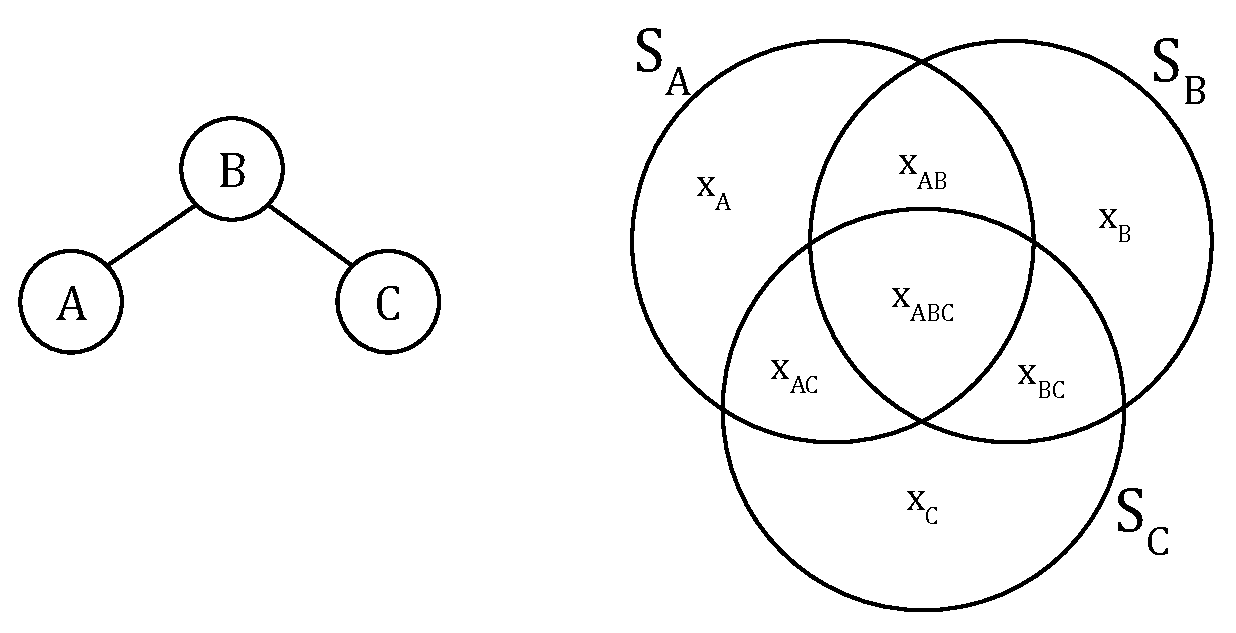
\includegraphics[scale=0.5]{figures/graphs_mhprove.pdf}
  \caption{Variáveis do problema de programação linear para um grafo de três vértices}
  \label{fig:graphs_mhprove}
\end{figure}

Definindo $\delta_A = 0,4$  e $\delta_B = 0,6$, é possível escrever o seguinte problema de programação linear inteira:
\begin{gather*}
\min \quad x_{A} + x_{B} + x_{AB} + x_{C} + x_{AC} + x_{BC} + x_{ABC} \\
\begin{aligned}
\textup{sujeito a} \quad 
6x_{A} + 6x_{B} - 4x_{AB} + 6x_{AC} + 6x_{BC} - 4x_{ABC} \leq 0 \\
-4x_{A} - 4x_{AB} - 4x_{C} + 6x_{AC} - 4x_{BC} + 6x_{ABC} \leq 0 \\
6x_{B} + 6x_{AB} + 6x_{C} + 6x_{AC} - 4x_{BC} - 4x_{ABC} \leq 0 \\
x_{A} + x_{AB} + x_{AC} + x_{ABC} \geq 1 \\
x_{B} + x_{AB} + x_{BC} + x_{ABC} \geq 1 \\
x_{C} + x_{AC} + x_{BC} + x_{ABC} \geq 1 \\
\end{aligned}
\end{gather*}

Cada variável $x_{S_1,\ldots,S_n}$ representa quantos elementos pertencem unicamente a $S_1 \cap \ldots \cap S_n$. A função objetivo é arbitrária e, assim sendo, escolhemos minimizar a quantidade de elementos distintos sendo usados. Cada restrição está associada a um par $x,y$ de vértices distintos do grafo. Caso eles sejam adjacentes, queremos que $J(x,y) \geq \delta_B$; caso contrário, que $J(S_x,S_y) \leq \delta_A$. A restrição surge diretamente da substituição das expressões de interseção e união implícitas em $J(S_x,S_y)$ pelas somas convenientes das variáveis. Por exemplo, a primeira restrição está associada aos vértices $A$ e $B$. Como eles são são adjacentes, eles devem cumprir
\[
    \frac{x_{AB} + x_{ABC}}{x_{A} + x_{B} + x_{AB} + x_{AC} + x_{BC} + x_{ABC}} \geq \frac{6}{10}
\] que resulta na restrição fornecida.

Uma solução deste problema se dá com $x_{AB} = 1$, $x_{BC} = 1$ e $x_{ABC} =1$, mostrando que uma construção para os parâmetros dados poderia ser, por exemplo, $S_A = \{1, 3\}$, $S_B = \{1, 2, 3\}$ e $S_C = \{2, 3\}$.

Ao aplicar a mesma ideia para o grafo bipartido completo $K_{3,3}$, para $\delta_A = 0,4$ e $\delta_B = 0,6$ (construção omitida por brevidade), é possível verificar que o problema não possui solução viável, demonstrando portanto a inviabilidade, para estes parâmetros da representação de grafos bipartidos. O mesmo ocorre em $K_{4,4}$, para $\delta_A = \frac{1}{3}$ e $\delta_B = \frac{1}{2}$, limites para os quais $K_{3,3}$ possui solução. É razoável então conjecturar se para quaisquer valores constantes de $\delta_A$ e $\delta_B$, com $\delta_B > \delta_A$, sempre haverá algum grafo bipartido que não é representável. Esta discussão fica em aberto para estudos futuros.

Com o intuito de encontrar uma representação probabilística com complexidade $o(n^2)$ bits, é possível modificar a ideia original para tornar o problema mais fácil.

É possível, por exemplo, ignorar as não-adjacências nos conjuntos independentes do grafo bipartido. Essa informação pode ser codificada como um bit a mais em cada vértice, para informar a qual conjunto independente o vértice faz parte. Assim o problema se resume a representar as adjacências e não-adjacências entre os conjuntos independentes apenas. Com essa modificação, a representação de grafos bipartidos, co-bipartidos e split pode ser exatamente igual, sendo necessária apenas a informação sobre qual tipo de grafo está sendo representado.

De fato, se existir representação probabilística eficiente para grafos bipartidos, é possível transformá-la numa representação para grafos gerais. Esta conclusão segue da transformação apresentada por Ford e Fulkerson em \cite{ford1962flows}. Seja $G' = (V', E')$ a transformação sobre um grafo $G = (V, E)$, tal que para cada vértice $v \in V$, existem $v_1, v_2 \in V'$ e para cada aresta $(u, v) \in E$ existe $(u_1, v_2) \in E'$. É fácil perceber que $G'$ é um grafo bipartido, com $|E'| = 2|E|$ e $|V'| = 2|V|$ (em particular, $G'$ é bipartido completo quando o $G$ é completo). Como existe aresta entre $u$ e $v$ em $G$ se e somente se existe aresta entre $u_1$ e $v_2$ em $G'$, então, se existir representação com $O(|V'| \log |V'|)$ bits para $G'$, esta representação também é eficiente em $G$, pois $O(|V'| \log |V'|) = O(2|V| \log 2|V|) = O(|V| \log |V|)$.